
This chapter presents a brief overview of the current implementation of \lang.
We developed a compiler and a virtual machine that runs
byte-code. The virtual machine for multicores makes use of the pthreads library.

\section{Overview}

The goal of our system is to keep the threads as busy as possible and to reduce inter-thread communication.
The load balancing aspect of the system is performed by our work scheduler that is based on a work
stealing algorithm. More specifically, threads can steal nodes of other threads to keep themselves busy.
Reduction of inter-thread communication is achieved by using a breadth-first search method to order nodes.

When the virtual machine starts, it reads the byte-code file and starts all threads.
As a first step, all threads will grab their nodes and assign the \texttt{owner} property of each node.
Because only one thread is allowed to do computation on the node at any giving time, this node's property
defines the thread with such permissions.
Next, we fill up the \emph{work queue} with the nodes we have picked. This queue
maintains the nodes that have new facts that need to be processed.

When a node sends a fact to another node, we need to check if the target node is not in the work queue of the owner thread.
If both nodes are in different threads, then we have a point of synchronization. At some point,
there will be no more work to do and the threads will go idle. There is a global atomic counter, a global
boolean flag and one boolean flag (active/idle) for each thread that are used to detect termination.
Once a thread goes idle, it decrements the global counter and changes its flag to idle. If the counter
goes to zero, the global flag is set to idle. Since every thread will be busy-waiting and checking
the global flag, they will detect the change and exit the program.

\section{Threads}

The work queue is actually implemented as two queues. First, there's one double-linked list for nodes
with priority equal to 0 called the \emph{normal queue}.
We use a double-linked list because it will be easier to move the node from this queue to the
\emph{priority queue}. The priority queue is an array based binary heap data structure that contains
all the unprocessed nodes with priority. To reduce the memory footprint of our queues, all the bookkeeping fields
such as the \texttt{next} and \texttt{prev} are part of the node data structure.
Each node also contains flags that indicate the queue where they are currently in and if they have facts to process.

\normalsize

\begin{comment}
\section{Nodes}

\begin{figure}[h!]
     \centering
   \resizebox{10cm}{!}{

    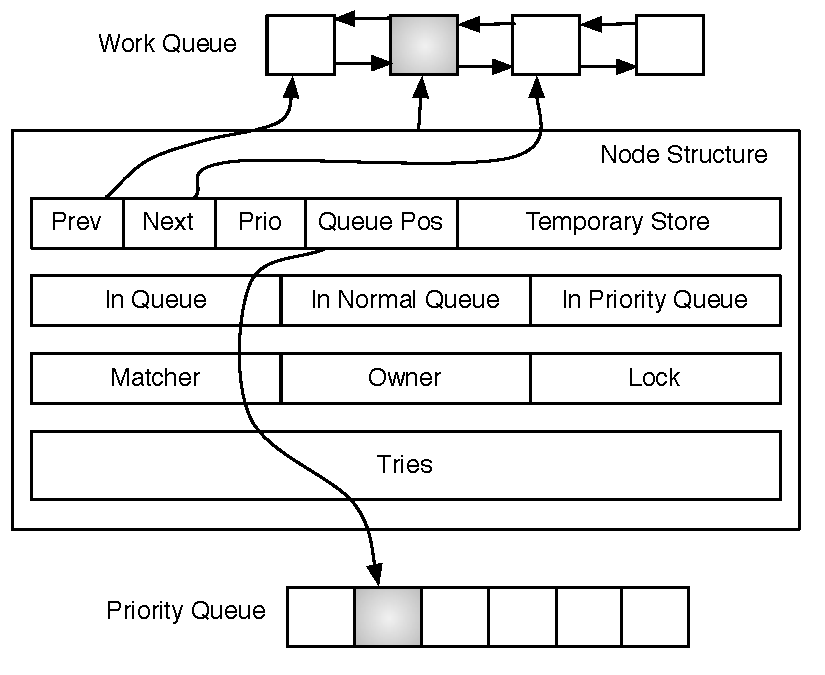
\includegraphics[width=0.5\textwidth]{node.pdf}}
    \caption{The node data structure.}
    \label{fig:node}
\end{figure}

The node data structure with an empty database occupies around 150 bytes.
In Fig.~\ref{fig:node} we present the node data structure and its fields. We summarize the data below:

\begin{description}
   \item[queue data]: Includes the field \texttt{Prev} (for the normal queue), \texttt{Next} (for the normal queue), \texttt{Prio} (priority) and \texttt{Queue Pos} (for the priority queue).
   \item[flags]: If the node is currently in the queue and in which queue. Includes \texttt{In Queue}, \texttt{In Normal Queue} and \texttt{In Priority Queue}.
   \item[temporary store]: A simple linked-list containing the unprocessed facts called \texttt{Temporary Store}.
   \item[database]: All the facts already processed which are true for this node. Is implemented as a trie and it is called \texttt{Tries}.
   \item[rule matcher]: The \texttt{Matcher} maintains the number of facts per predicate and which rules can be activated next. This is used for selecting the candidate rules.
   \item[owner]: Pointer to the owner thread. \texttt{Owner} in the figure.
   \item[lock]: A \texttt{Lock} mutex used to manipulate the node.
\end{description}
\end{comment}

\subsection{Work Stealing}

When a thread runs out of nodes to process, it will pick a thread at random and try to steal one node
from the target thread. The stealer thread will pop a node from either the priority queue or the normal queue. We use locks for mutual exclusion when dealing with those queues. Note that when a
node is stolen, its owner information also changes to the stealer thread.

It is important to note that whenever a node sends a coordination action fact to a node in another thread, the fact is ignored, due to the costs of sending
coordination data between threads. We intend to design an efficient mechanism to solve this problem.

In Fig.~\ref{code:work_loop} we present a simplified thread work loop that is executed in all threads. At each work cycle we check if thread has work in one of the two queues and if
not we attempt to steal a node from the other thread's queues. If our attempts to get some
work have succeeded, then we process the current node. Otherwise, the thread becomes idle and tries to synchronize and waits for the other threads to finish. Meanwhile, if the thread
receives some new node, \texttt{synchronize\_termination} will return \texttt{false} and
the thread will go to the next work cycle.

\begin{figure}[h!]
\small\begin{Verbatim}
void work_loop(thread_id tid) {
   while (true) {
      current_node = NULL;
      if(has_work(tid)) {
         current_node = pop_work(tid); // take node from one of the queues
      } else {
         // need to steal a node
         other = random_thread();
         current_node = steal_node_from_thread(other);
      }
      if(current_node == NULL) {
         become_idle(tid);
         if(synchronize_termination(tid))
            return;
         else
            become_active(tid);
      } else {
         process_node(current_node, tid);
      }
   }
}
\end{Verbatim}
  \caption{Thread work loop.}
  \label{code:work_loop}
\end{figure}

\section{Core Engine}\label{sec:core_engine}

Each node database is separated into two sets,
the database itself, and the \emph{temporary store}. The temporary store contains facts that have been
derived or have been sent to the node but have not been considered in rule derivations.
The temporary store exists for efficiency reasons because many linear facts are short-lived.

The temporary store is used to build the set of candidate rules that is represented as a priority queue.
To apply the rules, we take the highest priority rule from the queue and then run it.
If the derivation was successful, new facts may have been derived, thus we need to consider new
rules that are candidates from the newly derived facts and add them to the rule's priority queue.
On the other hand, when linear facts are consumed, some rules may not be applicable anymore and thus
we may need to remove them from the priority queue. In our implementation,
we keep a fact count for each predicate per node and also which predicates are needed for each rule. Whenever we have facts of some
predicates we can efficiently check if new rules are applicable for a specific node. We keep taking rules from the
queue until the queue is empty.

We do a small optimization to reduce the number of derivations of persistent facts. We
divide the program rules into two sets: \emph{persistent rules} and \emph{non persistent rules}.
Persistent rules are rules where only persistent facts are involved. We compile such rules
incrementally, that is, we attempt to fire all rules where a persistent fact is used. This is called
the \emph{pipelined semi-naive} evaluation and it originated in the P2 system~\cite{Loo-condie-garofalakis-p2}.
This evaluation method avoids excessing re-derivations of the same fact. The order of derivation does not matter for those rules, since
only persistent facts are used.

\section{Database}

The database is implemented using the trie data structure. Tries are trees where facts are indexed
by the common arguments. Because we need to delete facts from the database, we implement each trie level
as a double linked list so trie nodes can be easily removed. If a trie level has too many nodes, we
transform the linked list into a hash table in order to improve lookup.

Each node uses a trie per predicate to store facts. During matching of rules, we build a
\emph{match object}, which matches some arguments of the target predicate to instantiated values, so
that by searching the predicate trie from top to bottom, we can easily discard invalid trie branches.

\section{Summary}

This section provided a very brief overview of the current implementation of \lang. Although the parallel
and load balancing facilities of the runtime system are mostly completed, there is still some
implementation work to be done at the core engine level in order to make execution faster.
As it will be explained in Chapter~\ref{chapter:exp}, \lang is not yet competitive against
other systems, therefore we intend to perform more implementation work as part of this
thesis to make the virtual machine as fast as possible.